\documentclass[a4paper,12pt]{book}

%%%%%%%%%%%%%%%%%%%%%%%%%%%%%%%%%%%
%\input{preamble}

\usepackage[english]{babel}

\usepackage{anyfontsize}

\usepackage{microtype}
\usepackage{amssymb}
\usepackage{amsmath} % for \text macro
\usepackage{mathabx}
\usepackage{graphicx}

%%%%% Fonts %%%%%%
%\input Eichenla.fd
%\newcommand*\initfamily{\usefont{U}{Eichenla}{xl}{n}}

\input Elzevier.fd
\newcommand*\initfamily{\usefont{U}{Elzevier}{xl}{n}}
%%%%% %%%%%%%%%

\usepackage{fancyhdr}
\pagestyle{fancy}
\fancyhf{}
\renewcommand{\headrulewidth}{0pt}
\fancyfoot[CO]{\hrulefill\ \textbf{[\thepage]} \hrulefill}
\fancyfoot[CE]{\hrulefill\ \textbf{[\thepage]} \hrulefill}

\addto\captionsenglish{
	\renewcommand{\contentsname}{Table of Contents}
}

\usepackage{tikz}

% Changing the Chapter and section style
\usepackage{titlesec}
\titleformat{\chapter}[display]{\Huge}{}{0em}{}
\titlespacing{\chapter}{0pt}{0pt}{15pt}
\titleformat{\section}{\normalfont\sffamily\bfseries}{}{0em}{}
\titlespacing{\section}{0em}{2em}{1.5em}

%Setting Paragraph lengths
%\setlength{\parskip}{0em}
%\setlength{\parindent}{0em}

\usepackage{rotunda}
%\usepackage{rustic} rust font
%\usepackage{fonts} gothic font

% The style of the solution text
\newcommand{\solution}[1]{{\itshape #1}}

% The style of the problem text including the background
\newcommand{\problemdef}[1]{\noindent\section[Problem \arabic{section}]{%
\begin{tikzpicture}[transform shape, every node/.style={inner sep=0,outer sep=0}]%
\node [draw=white, fill=white, rectangle, inner xsep=26pt, inner ysep=20pt] (box) {%
\begin{minipage}[h!]{0.86\textwidth}%
#1%
 \end{minipage} %
};%
\node[overlay, anchor=north west] at (box.north west) {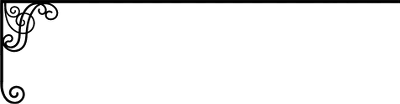
\includegraphics[width=.40\textwidth]{QuestionCorner.png}};
\draw[line width=2pt] (box.north west) -- ++(0:250pt);      
\draw[line width=2pt] (box.north west) -- ++ (270:43pt);
\draw (box.south east) -- ++(90:37pt);
\draw (box.south east) -- ++(180:100pt);
\end{tikzpicture}%
}}

\newcommand{\scriptedtitle}[3]{%
\raisebox{-45pt}{{\fontsize{80}{100}\selectfont\initfamily #1}}%
{\rtndfamily#2}%
\hspace{8pt}\raisebox{-45pt}{{\fontsize{100}{120}\selectfont #3}}%
}

\newcommand{\stylizedchaptertitle}[4]{
\scriptedtitle{#1}{#2}{#3}\\%
\vspace{7pt}%
\hrule height 2pt% 
\vspace{2pt}%
\hrule%
\vspace{2pt}%
\hfill{\rtndfamily #4}%
\hrule height 1pt%
\vspace{2pt}%
\hrule%
\vspace{20pt}%
\hfill$\bigstar$\hfill%
}


\usepackage{hyperref}
%%%%%%%%%%%%%%%%%%%%%%%%%%%%%%%%%%%

\begin{document}
% Create the title page
\title{Solutions for Rudin's Principles of Mathematical Analysis}
\author{Andrew Rickert}
\date{\today}
\maketitle

% Add the table of contents
\tableofcontents
\thispagestyle{empty}

%%%%%%%%% Chapter 2 %%%%%%%%%%%%%%
\chapter[Chapter 1: The Real and Complex Number Systems]{\stylizedchaptertitle{C}{hapter}{1}{The Real and Complex Number Systems}}
\thispagestyle{fancy}

\problemdef{If $r$ is rational $(r \neq 0)$ and $x$ is irrational, prove that $r + x$ and $rx$ are irrational}

\solution{%
If $r+x = s$ is rational then $x = (r+x)-r = s - r$ is rational since $-r$ is rational and the rationals are closed. This is contradiction which shows that $r+x$ can not be rational.\\
\indent The proof for $rx$ is similar since $\frac{1}{r}$ is rational. Because the rationals are closed we have $x = \frac{1}{r}\cdot(rx)$ as a rational since it is the product of two rationals. This contradiction establishes the result.
}

\problemdef{Prove that there is no rational number whose square is 12}

\solution{%
We first prove the preliminary result that $3 \mid m^2$ implies $3 \mid m$.
We suppose that it is not the case the $3 \mid m$, this would mean that $m = 3k+1$ or $m = 3k+2$ where $k \in \mathbb{N}$.\\
\indent In the first case we see that $m^2 = 9k^2 + 6k + 1$ which is not divisible by 3. We can see this showing that divisibility by 3 is not possible. Let $m^2 = 3 q$ since we are assuming divisibility. We calculate:
\begin{eqnarray*}
3 q &=& m^2 \\
3 q &=& 9k^2 + 6k + 1 \\
3 q &=& 3 (3k^2 + 2 k) + 1 \\
3 q &=& 3 p + 1 \quad \text{p is clearly an integer}\\
3 (q - p) &=& 1
\end{eqnarray*}
Since $\frac{1}{3}$ is not an integer the final relation is an impossibility. This shows that $3 \nmid m^2$ if $m = 3 k +1$. The argument that $3 \nmid m^2$ if $m = 3 k + 2$ is analogous.
\indent Both of the possibilities for $m$ not being divisible by 3 lead to contradictions with the hypothesis that $3 \mid m^2$. This establishes the preliminary result.\\
\indent If we know that $x = \sqrt{3}$ is irrational then by problem 1, we know that $2\cdot \sqrt{3}$ is also irrational. In other words, if there are no $m,n$ such that $\frac{m}{n} = 2 \cdot \sqrt{3}$ then there is no $(\frac{m}{n})^2 = 4 \cdot 3 = 12$. Thus we only need to prove that $\sqrt{3}$ is irrational to finish the problem.\\

We assume that there exists $m,n$ such that $3 = \frac{m^2}{n^2}$ where $m$ and $n$ have no common factors.\\
\indent Since $3 n^2 = m^2$ we have $m^2$ is divisible by 3. The preliminary result allows us to infer that $3 \mid m$ so $m = 3 k$. Substituting gives $3n^2 = (3k)^2 = 9k^2$.\\
\indent The previous relation says that $3 \mid n^2$ which, again by the preliminary result, shows that $3 \mid n$.\\

Since both $m$ and $n$ are divisible by 3 they have a factor in common which contradicts the assumption of that $m$ and $n$ shared no common factor. The contradiction establishes that 12 must be irrational.
}

\problemdef{Prove Proposition 1.15}

\solution{%
The proof is the same as Proposition 1.14 but with $+$ substituted \newline for $\cdot$ (multiplication) and 0 substituted for 1.
}

\problemdef{Let $E$ be a nonempty subset of an order set; suppose $\alpha$ is a lower bound of $E$ and $\beta$ is an upper bound of $E$. Prove that $\alpha \le \beta$}

\solution{%
Given that $\alpha$ is a lower bound we know that $\alpha \le x$ for all $x \in E$. This means for a given $x' \in E$ we have $\alpha \le x'$. \\
\indent We also know that $\beta$ in a upper bound and therefore $x \le \beta$ for all $x \in E$. Thus we have 
\[
	\alpha \le x' \le \beta
\]
}

\problemdef{Let $A$ be a nonempty set of real numbers which is bounded below. Let $-A$ be the set of all numbers $-x$, where $x \in A$. Prove that
\[
	\text{inf}\ A = -\text{sup} (-A)
\]}

\solution{%
Let $\alpha = \text{inf}\ A$. From this we have that $\alpha \le x$ for all $x \in A$ but this means $-x \le -\alpha$ for all $-x \in -A$. With $-\alpha$ established as an upper bound on $-A$ the final step is to show that is the least upper bound.\\
\indent Let's assume that there exists a $\beta$ such that $-x \le -\beta$ for all $x \in A$ and $-\beta < -\alpha$. Thus, $-\beta$ is an upper bound for $-A$ but because $\beta \le x$ for all $x \in A$ we know $\beta$ is a lower bound for $A$. $-\beta < -\alpha$ implies $\alpha < \beta$ which is a contradiction because $\alpha$ is the greatest lower bound. \\
\indent We have established there is no lower bound of $-A$ that is lower than $-\alpha$ so $-\text{inf}\ A = -\alpha = \text{sup}\ ({-A})$.
}

%%%%%%%%% Chapter 2 %%%%%%%%%%%%%%
\chapter[Chapter 2: Basic Topology]{\stylizedchaptertitle{C}{hapter}{2}{Basic Topology}}
\thispagestyle{fancy}

\problemdef{Prove that the empty set is the subset of the every set}

\solution{To say that $\emptyset \subset A$ is to say if $x \in \emptyset$ then $x \in A$. By definition the antecedent $x \in \emptyset$ is false which means the if-then statement as a whole is true. This establishes the conclusion. }

\problemdef{A complex number $z$ is said to be \emph{algebraic} if there are integers $a_0, \cdots, a_n$, not all zero, such that
\[
	a_o z^n + a_1 z^{n-1} + \cdots + a_{n-1} z + a_n = 0
\]
Prove that the set of all algebraic numbers is countable.
}

\solution{Prove it}

\problemdef{Prove that there exist real numbers that are not algebraic}

\solution{It was shown in the previous problem that the algebraic numbers are countable. We also know from theorem 2.43 that perfect sets are uncountable and it is clear $\mathbb{R}$ is a perfect set. 

We may logically divide the reals $\mathbb{R}$ into the algebraic and the non-algebraic numbers. If non-algebraic numbers did not exist than the algebraic numbers would be all of $\mathbb{R}$ which implies $\mathbb{R}$ is countable.

The contradiction implies there must be non-algebraic numbers and further, there must be uncountably many of them.}

\problemdef{Is the set of all irrational real numbers countable?}

\solution{%
No. \\
\indent The real numbers can be divided into the rationals and those that are not rational i.e. the irrationals. If we suppose that the irrationals are countable then the union of the rationals and the irrationals is also countable since it is a union of countable sets (Theorem 2.12).\\
\indent The real numbers are a perfect set and are therefore uncountable so it is not the case the irrationals are countable otherwise the reals would be as well.
}

\problemdef{Construct a bounded set with exactly three limit points}

\solution{%
Let 
\begin{eqnarray*}
E_1 &=& \{ 1 + \frac{1}{n}\ |\ n \in \mathbb{N} \} \\
E_5 &=& \{ 5 + \frac{1}{n}\ |\ n \in \mathbb{N} \} \\
E_9 &=& \{ 9 + \frac{1}{n}\ |\ n \in \mathbb{N} \}
\end{eqnarray*}

If we define $E = E_ 1 \cup E_5 \cup E_9$ then $E$ is the set with the desired properties.
}


\problemdef{Let $E'$ be the set of all limit points of a set $E$. Prove that $E'$ is closed. Prove that $E$ and $\overline{E}$ have the same limit points. (Recall that $\overline{E} = E \cup E'.$) Do $E$ and $E'$ always have the same limit points?}

\solution{%
We will prove that $E'$ is closed by showing it's complement is open.\\
\indent Let $x \in (E')^c$. Because $x \notin E'$ we know that $x$ is not a limit point and there exists a neighborhood of $x$, $N(x)$, such that $N(x) \cap E = \emptyset$. With no elements of $E$ in $N(x)$ we know there also must be no limit points in $N(x)$ so $N(x) \subset (E')^c$ which shows $(E')^c$ is open.\\

\indent To show that $E$ and $\overline{E}$ have the limit points we first note that if $x \in E'$ then every neighborhood of $x$ contains an element of $E$. Since $E \subset \overline{E}$ we know that every neighborhood of $x$ contains a point of $\overline{E}$. That is, $x$ is a limit point of $\overline{E}$.\\
\indent The question is whether a limit point of $\overline{E}$ is a limit point of $E$. To show this we let $x$ be a limit point $\overline{E}$. If $N(x)$ is neighborhood of $x$ then every neighborhood contains either a point $y \in E$ or a point $y \in E'$. In the second case we note that since $N(x)$ is open there exists a neighborhood around $y$ such that $N(y) \subset N(x)$. Because $y \in E'$ we know that the neighborhood $N(y)$ contains a point of $E$. So, we know that in all cases a neighborhood of $x$, the limit point of $\overline{E}$, will contain a point of $E$ meaning $x$ is a limit point of $E$.\\

The sets $E$ and $E'$ don't have the same limit points. To see this let  $E = \{1, \frac{1}{2}, \frac{1}{3}, \dots \}$. The set has a limit point $\{ 0 \}$  but $E' = \{ 0 \}$ has no limit points.
}

\problemdef{Let $A_1, A_2, A_3, \dots$ be subsets of a metric space.\\
(a) If $B_n = \cup^n_{i = 1} A_i$, prove that $\overline{B_n} = \cup^n_{i = 1} \overline{A}_i$, for $n = 1,2,3,\dots$\\
(b) If $B_n = \cup^\infty_{i = 1} A_i$, prove that $\overline{B_n} \supset \cup^\infty_{i = 1} \overline{A}_i$\\
Show, by example, that this inclusion can be proper.
}

\solution{%
The first part of the problem ultimately hinges on showing that \\$(A_1 \cup A_2)' = A_1' \cup A_2'$ so we show this first.\\
\indent If $x \in A_1' \cup A_2'$ then $x$ is either a limit point of $A_1$ or $A_2$. We may suppose that $x \in A_1$ but this means that every neighborhood of $x$ contains an element $y \in A_1$ therefore $y \in A_1 \cup A_2$. This says that every neighborhood contains an element of $A_1 \cup A_2$ so $x$ is a limit point of $A_1 \cup A_2$. The same logic follows if $x \in A_2$ and we get $(A_1 \cup A_2)' \supset A_1' \cup A_2'$.\\
\indent Going the other direction. Suppose that $x \in (A_1 \cup A_2)' $ so every neighborhood of $x$ contains a point of $A_1 \cup A_2$. Each neighborhood will contain a point $y \in A_1$ or $y \in A_2$. Since this is the case for every neighborhood it must be true that $x$ is a limit point of either $A_1$ or $A_2$. If this were not the case then there would exist a neighborhood of $x$ that did not contain a point of either $A_1$ or $A_2$ but then $x$ would not be a limit point of $A_1 \cup A_2$. This contradiction implies that $x \in A_1'$ or $x \in A_2'$ so $x  \in A_1' \cup A_2 '$ and we get $(A_1 \cup A_2)' \subset A_1' \cup A_2'$ showing that $(A_1 \cup A_2)' = A_1' \cup A_2'$. \\

We now prove part a by induction. For $n = 1$ the theorem is trivially true. For $n = 2$ we calculate
\begin{eqnarray*}
\overline{B_2} &=& \overline{A_1 \cup A_2}\\
 &=& (A_1 \cup A_2) \cup (A_1 \cup A_2)' =  (A_1 \cup A_2) \cup (A_1' \cup A_2') \quad \text{by the previous remarks}\\
 &=& (A_1 \cup A_1') \cup (A_2 \cup A_2') =  \overline{A_1} \cup \overline{A_2}\\
\end{eqnarray*}

We may assume the induction hypothesis $\overline{B_{n-1}} = \cup^{n-1}_{i = 1} \overline{A_i}$ and consider the case for $n$
\begin{eqnarray*}
\overline{B_n} &=& \overline{\cup^n_{i = 1} A_i} \\
&=& \overline{\cup^{n-1}_{i = 1} A_i} \cup \overline{A_n} \quad \text{since we proved the case for $n = 2$} \\
&=& \cup^{n-1}_{i = 1} \overline{A_i} \cup \overline{A_n} \quad \text{by the induction hypothesis}\\
&=& \cup^n_{i = 1} \overline{A_i}
\end{eqnarray*}
This completes the induction and finishes part a.\\

For part b of the problem we only need to show 
}

\problemdef{Is every point of every open set $E \subset \mathbb{R}^2$ a limit point of $E$? Answer the same question for closed sets in $\mathbb{R}^2$}

\solution{%
Yes, every point of an open set in $\mathbb{R}^2$ is a limit point. \\
\indent Because $E$ is an open set there is a neighborhood, $N_r(x),\ $around $x \in E$ such that $N_r(x) \subset E$. Let $x = (x_1, x_2) \in \mathbb{R}$. By the archimedean property we know that between $(x_1, x_2)$ and $(x_1+r,x_2)$ there is a rational number $q$ such that $x_1 < q < x_1 + r$ so $(q,x_2) \in N_r(x)$ and $(q,x_2) \in E$. So the neighborhood contains a point of $E$.\\
\indent Every neighborhood of a larger radius $s > r$ is such that $N_r(x) \subset N_s(x)$ so $N_s(x)$ also contains a point of $E$. \\
\indent If the neighborhood is of a radius $p < r$ then we can use the same archimedean argument above to find a point $y \in N_q(x)$ and $y \in E$.\\

Every point of a closed set in $\mathbb{R}$ is not a limit point. Consider the set $E = \{ (0,0)\} \cup \{ (x,0) \ |\ x \in [1,2]\}$. We have a closed set with an isolated point and a line segment. If we surround $y = (0,0)$ with the neighborhood $N_{1 / 2}(y)$ then the neighborhood does not intersect with $E$ except for $y$ itself which shows $(0,0)$ is not a limit point.
}

\problemdef{%
Let $E^\circ$ denote the set of all interior points of a set $E$.\\
(a) Prove that $E^\circ$ is always open\\
(b) Prove that $E$ is open if and only if $E^\circ = E$\\
(c) If $G \subset E$ and $G$ is open, prove that $G \subset E^\circ$\\
(d) Prove that the complement of $E^\circ$ is the closure of the complement of $E$\\
(e) Do $E$ and $\overline{E}$ always have the same interiors?\\
(f) Do $E$ and $E^\circ$ always have the same closures?
}

\solution{%
\noindent (a) If $x \in E^\circ$ then we know that there is a neighborhood $N(x)$ such that $N(x) \subset E$. Since $N(x)$ is open we know that $y \in N(x)$ means there is a neighborhood $N(y) \subset N(x)$ implying $N(y) \subset E$ giving us $y \in E^\circ$. This shows that $N(x) \subset E^\circ$ which produces the necessary open set contained in $E^\circ$.
\noindent (b) The previous part shows that $E^\circ = E$ implies that $E$ is open so we only need to show the reverse claim.
}

%%%%%%%%% Chapter 3 %%%%%%%%%%%%%%
\chapter[Chapter 3: Numerical Sequences and Series]{\stylizedchaptertitle{C}{hapter}{3}{Numerical Sequences and Series}}
\thispagestyle{fancy}
\problemdef{Stuff}

%%%%%%%%% Chapter 3 %%%%%%%%%%%%%%
\chapter[Chapter 4: Continuity]{\stylizedchaptertitle{C}{hapter}{4}{Continuity}}
\thispagestyle{fancy}


\appendix
\addtocontents{toc}{\bigskip}
\addcontentsline{toc}{part}{Appendix}

\end{document}
